\documentclass[12pt, a4paper]{article}  


\usepackage{amsmath,amsfonts,amssymb,amsthm,mathtools}  
\usepackage{graphicx}

\usepackage{fontspec}         
\setmainfont{Phorssa} 
\newfontfamily{\cyrillicfonttt}{Phorssa}
\newfontfamily{\cyrillicfont}{Phorssa}
\newfontfamily{\cyrillicfontsf}{Phorssa}   

\usepackage{unicode-math}  
\setmathfont{Asana-Math.otf}   
 

\usepackage{polyglossia}      
\setdefaultlanguage{russian}  
\setotherlanguage{english} 
\usepackage{graphicx}                  
\usepackage{graphics} 
\usepackage{wrapfig}

\begin{document}

Советую не вводить штрафы \newline за просроченные дз- иначе быть вам  с Кафидычем,
\begin{wrapfigure}[10]{r}{0.3\linewidth} 

\includegraphics[width=\linewidth]{rev1.png}
\end{wrapfigure}
 который изо дня в день из месяца в месяц из года в год будет читать вам лекцию об объекте и субъекте, а при этом вы будете вновь и вновь конспектировать ПБУ. 
\begin{flushright}
Ваши недоброжелатели
\end{flushright}
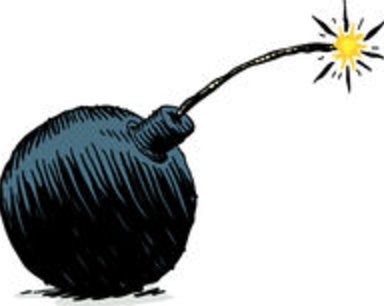
\includegraphics[scale=0.5]{bmb.png}
\end{document}